\begin{figure*}[t]
 \begin{center}
  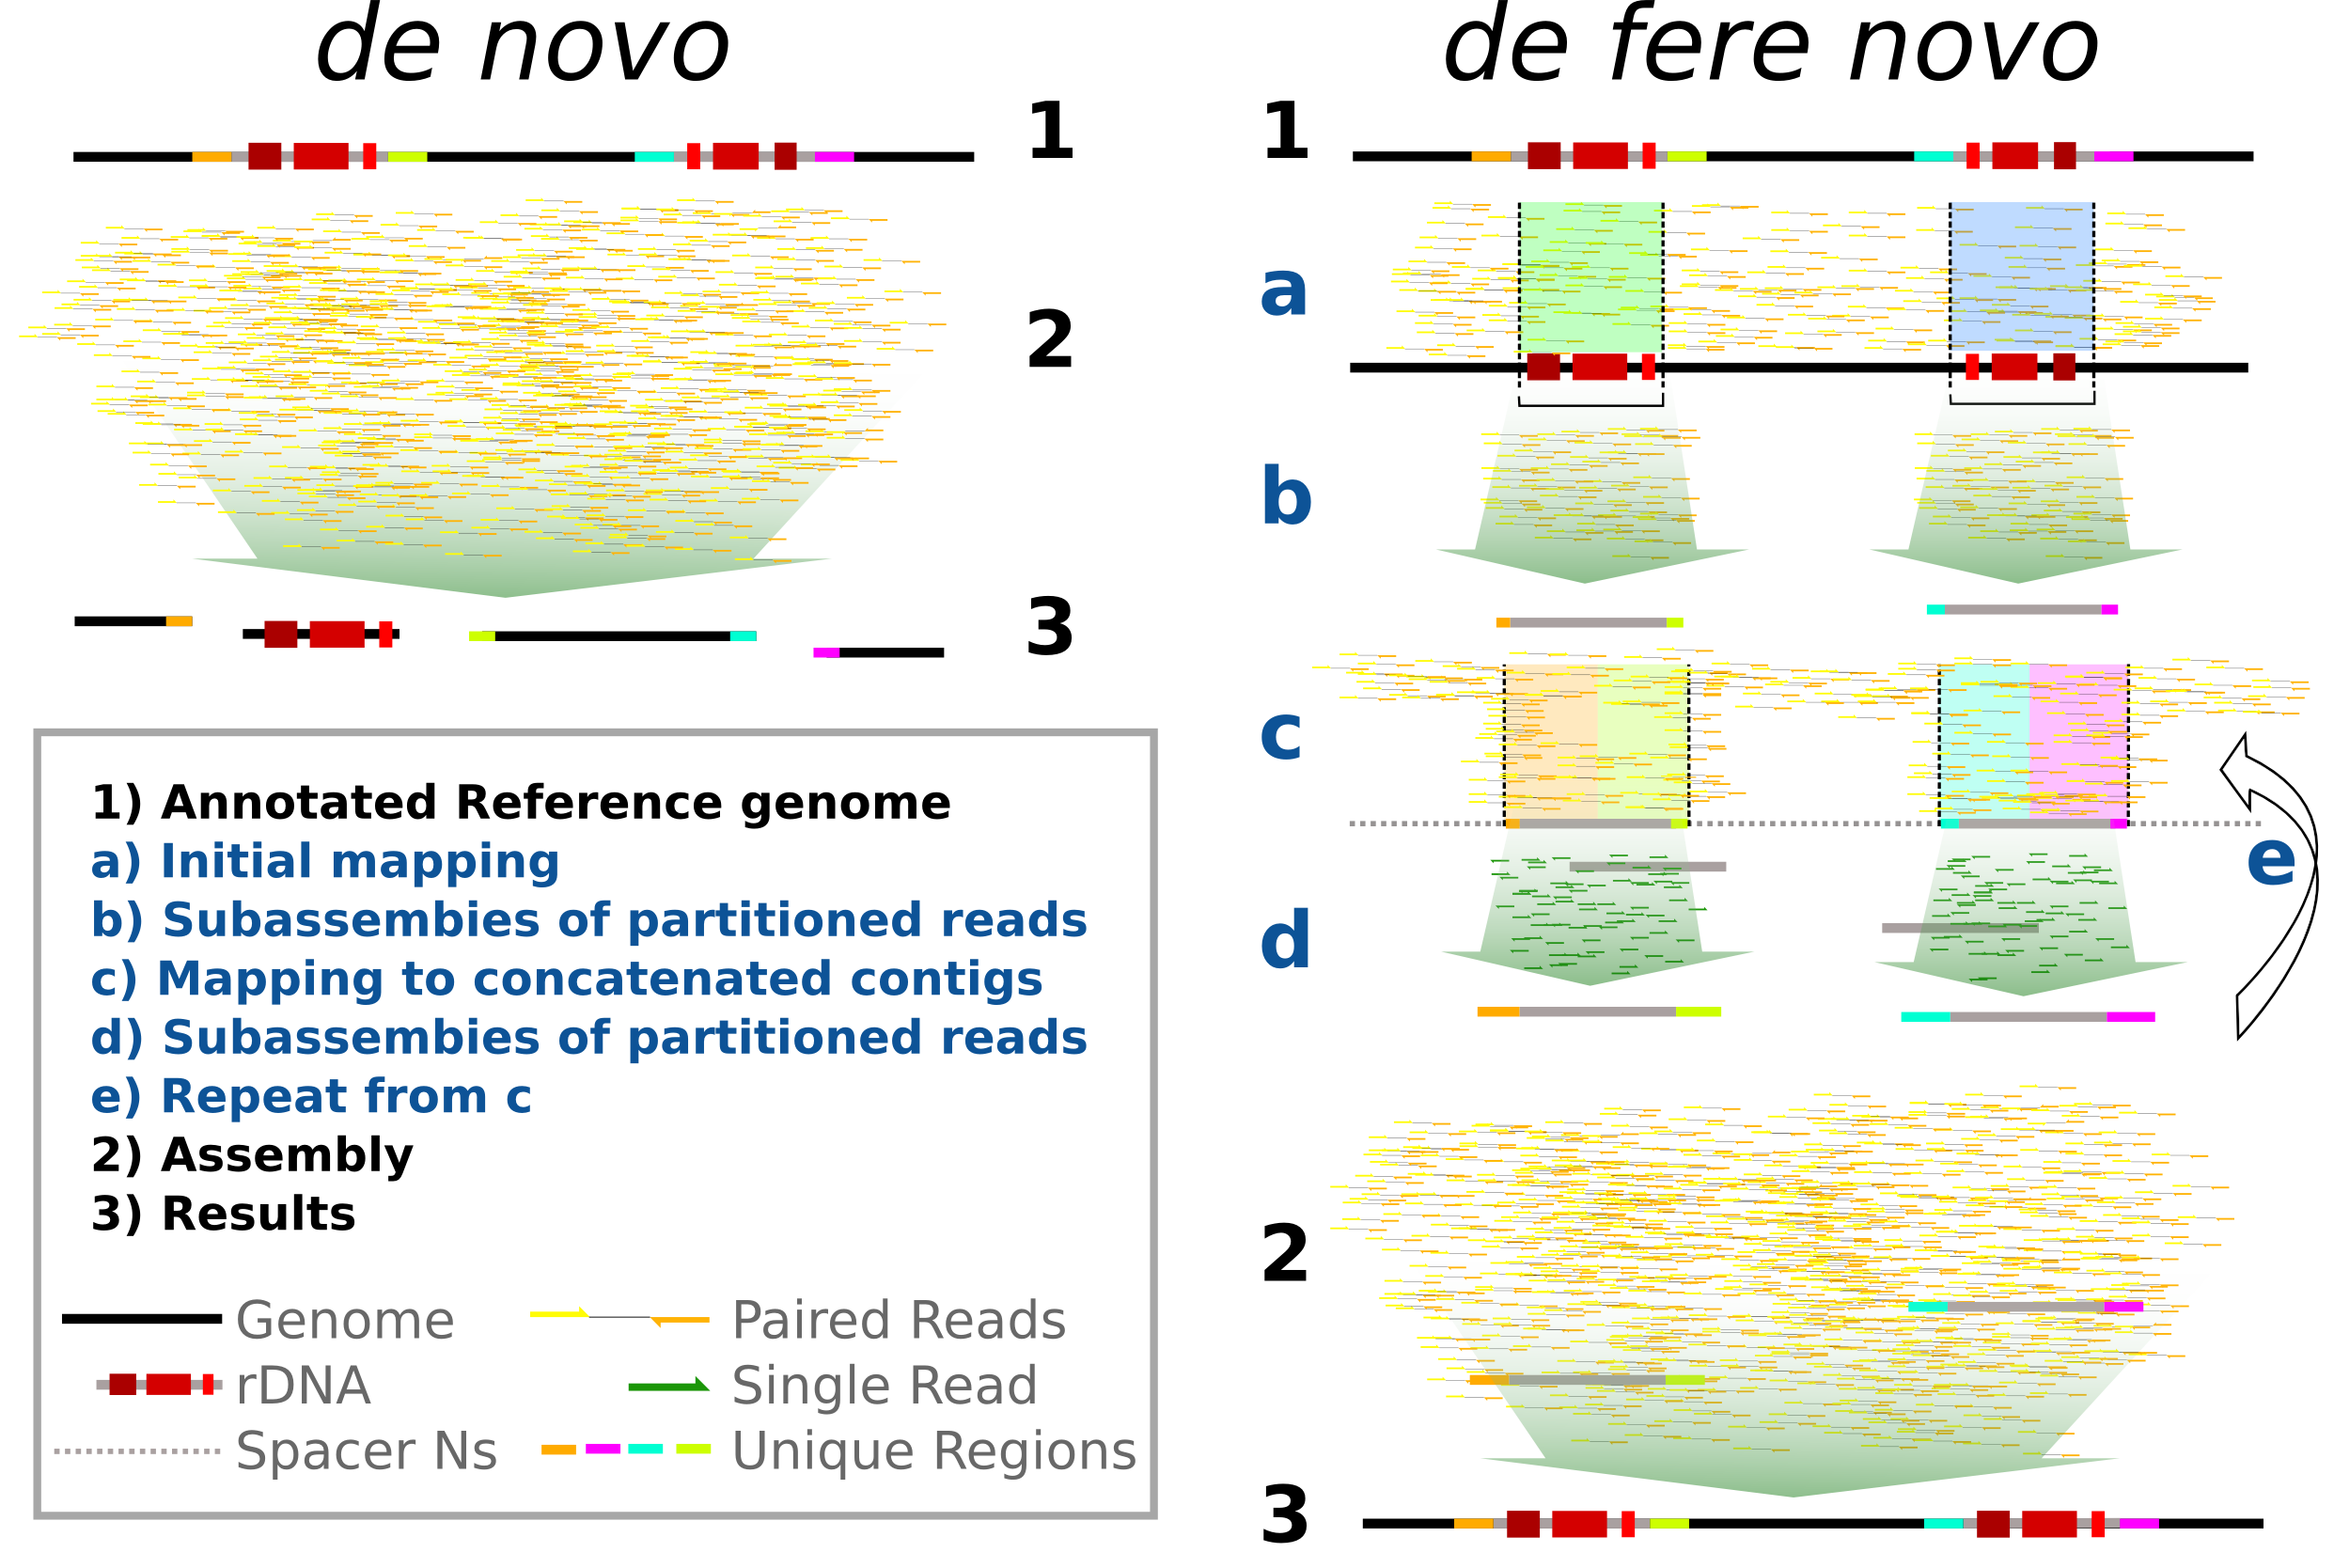
\includegraphics[width=.85\textwidth]{riboSeed_v14}
  \end{center}
  \caption{A comparison of \textit{de novo} assembly to \textit{de fere novo} assembly, as implemented in riboSeed. In riboSeed, reads are mapped to a reference genome, and those reads that align to rDNA and flanking regions are extracted. A subassembly for each group of reads that maps to an rDNA region is constructed to produce a ``pseudocontig'' for each region. These pseudocontigs are concatenated together separated by 1kb of Ns as a spacer. Reads are then iteratively mapped to the concatenated pseudocontigs, extracted, and again subassembled to each region. After the final iteration, the pseudocontigs are included with raw reads in a standard \textit{de novo} assembly. The subassemblies attempt to bridge proper rDNA regions by ensuring that flanking regions (represented here by colors) remain correctly paired. The \textit{de novo} assembly collapses the rDNAs, but \textit{de fere novo} places the rDNAs in the proper genomic context.
  }
  \label{fig:overview}
\end{figure*}
